% diagrammatic_calculus.tex
% LaTeX counterpart of docs/diagrammatic_calculus.md
% Section §3.5

\section{Diagrammatic Calculus}\label{sec:diagrammatic-calculus}

\begin{assumption}\label{ass:diagrammatic}
\begin{enumerate}[label=(A3.5.\arabic*)]
    \item Fusion category $(\catC, \otimes, \one)$ over $k = \mathbb{C}$ (Definition~\ref{def:fusion-category}).
    \item $\catC$ is pivotal (left and right duals agree).
    \item All diagrams are read bottom-to-top (source at bottom, target at top).
\end{enumerate}
\end{assumption}

\subsection{String Diagrams for Morphisms}\label{sec:string-diagrams}

String diagrams provide a graphical calculus for computations in monoidal categories. Rather than manipulating algebraic expressions, we draw pictures that encode the same information but make certain properties (like coherence) manifest.

\begin{definition}[String diagram]\label{def:string-diagram}
A \emph{string diagram} in a monoidal category represents morphisms graphically according to the following rules:
\begin{enumerate}
    \item \textbf{Objects:} Represented by labelled vertical strings (lines).
    \item \textbf{Morphisms:} A morphism $f: A \to B$ is drawn as a node (box or vertex) with input string $A$ entering from below and output string $B$ exiting above.
    \item \textbf{Composition:} The composite $g \circ f$ (first $f$, then $g$) is drawn by stacking $g$ above $f$.
    \item \textbf{Tensor product:} The tensor $f \otimes g$ is drawn by placing $f$ and $g$ side-by-side, with $f$ on the left.
    \item \textbf{Identity:} The identity morphism $\mathrm{id}_A: A \to A$ is a straight vertical line labelled $A$.
\end{enumerate}
\end{definition}

\begin{figure}[ht]
\centering
\begin{tikzpicture}[scale=0.8]
    % Identity morphism
    \begin{scope}[xshift=0cm]
        \draw[thick] (0,0) -- (0,2);
        \node[left] at (0,1) {$A$};
        \node at (0,-0.5) {$\mathrm{id}_A$};
    \end{scope}

    % Single morphism
    \begin{scope}[xshift=3cm]
        \draw[thick] (0,0) -- (0,0.7);
        \draw[thick] (0,1.3) -- (0,2);
        \node[morphism box] at (0,1) {$f$};
        \node[left] at (0,0.35) {$A$};
        \node[left] at (0,1.65) {$B$};
        \node at (0,-0.5) {$f: A \to B$};
    \end{scope}

    % Composition
    \begin{scope}[xshift=7cm]
        \draw[thick] (0,0) -- (0,0.5);
        \draw[thick] (0,1.1) -- (0,1.4);
        \draw[thick] (0,2) -- (0,2.5);
        \node[morphism box small] at (0,0.8) {$f$};
        \node[morphism box small] at (0,1.7) {$g$};
        \node[left] at (0,0.25) {$A$};
        \node[left] at (0,2.25) {$C$};
        \node at (0,-0.5) {$g \circ f$};
    \end{scope}

    % Tensor product
    \begin{scope}[xshift=11cm]
        \draw[thick] (-0.5,0) -- (-0.5,0.7);
        \draw[thick] (-0.5,1.3) -- (-0.5,2);
        \draw[thick] (0.5,0) -- (0.5,0.7);
        \draw[thick] (0.5,1.3) -- (0.5,2);
        \node[morphism box small] at (-0.5,1) {$f$};
        \node[morphism box small] at (0.5,1) {$g$};
        \node at (0,-0.5) {$f \otimes g$};
    \end{scope}
\end{tikzpicture}
\caption{Basic string diagram elements: identity, morphism, composition, and tensor product.}
\label{fig:string-basics}
\end{figure}

\begin{convention}[Reading order]\label{conv:reading-order}
Throughout this paper, string diagrams are read \textbf{bottom-to-top} (inputs at bottom, outputs at top) and tensor factors are ordered \textbf{left-to-right}. This follows the categorical convention where composition $g \circ f$ means ``first $f$, then $g$''.
\end{convention}

For fusion categories, strings are labelled by simple objects $X_i \in \Irr(\catC)$.

\begin{remark}[Interchange law]
The string diagram calculus automatically encodes the \emph{interchange law}: for composable morphisms $f_1: A_1 \to B_1$, $g_1: B_1 \to C_1$, $f_2: A_2 \to B_2$, $g_2: B_2 \to C_2$,
\begin{equation}
    (g_1 \otimes g_2) \circ (f_1 \otimes f_2) = (g_1 \circ f_1) \otimes (g_2 \circ f_2).
\end{equation}
Diagrammatically, this is manifest: both sides describe the same picture of $f_1, f_2$ below and $g_1, g_2$ above.
\end{remark}

\begin{citationblock}
Selinger, \emph{A survey of graphical languages for monoidal categories}, in \emph{New Structures for Physics}, Springer (2011), \S4 \unverified
\end{citationblock}

\subsection{Isotopy and Pivotal Structure}\label{sec:isotopy-pivotal}

\begin{definition}[Isotopy invariance]\label{def:isotopy}
String diagrams satisfy \emph{isotopy invariance}: continuously deforming a diagram without crossing strings or moving nodes past each other yields the same morphism. This is a consequence of the coherence theorem for monoidal categories.
\end{definition}

\begin{definition}[Pivotal category]\label{def:pivotal}
A \emph{pivotal structure} on a rigid monoidal category provides:
\begin{enumerate}
    \item A natural isomorphism $X \cong X^{**}$ (double dual) for each object $X$.
    \item Consistency between left and right duals.
\end{enumerate}
In a pivotal fusion category, upward and downward strands are related by duality:
\begin{itemize}
    \item Upward-oriented strand labelled $X$: the object $X$.
    \item Downward-oriented strand labelled $X$: the dual object $X^*$.
\end{itemize}
\end{definition}

\begin{figure}[ht]
\centering
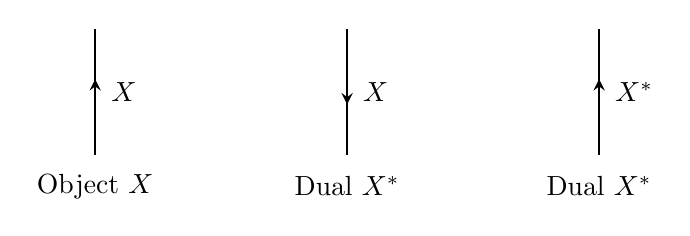
\begin{tikzpicture}[scale=0.8]
    % Upward strand = X (arrow pointing up)
    \begin{scope}[xshift=0cm]
        \draw[thick] (0,0) -- (0,2);
        \draw[thick,->,>=stealth] (0,0.8) -- (0,1.2);
        \node[right] at (0.1,1) {$X$};
        \node at (0,-0.5) {Object $X$};
    \end{scope}

    % Downward strand = X^* (arrow pointing down)
    \begin{scope}[xshift=4cm]
        \draw[thick] (0,0) -- (0,2);
        \draw[thick,->,>=stealth] (0,1.2) -- (0,0.8);
        \node[right] at (0.1,1) {$X$};
        \node at (0,-0.5) {Dual $X^*$};
    \end{scope}

    % Equivalently, X* labelled going up
    \begin{scope}[xshift=8cm]
        \draw[thick] (0,0) -- (0,2);
        \draw[thick,->,>=stealth] (0,0.8) -- (0,1.2);
        \node[right] at (0.1,1) {$X^*$};
        \node at (0,-0.5) {Dual $X^*$};
    \end{scope}
\end{tikzpicture}
\caption{In pivotal categories, strand orientation distinguishes $X$ from $X^*$.}
\label{fig:pivotal-strands}
\end{figure}

\begin{consequence}
Pivotal structure allows ``bending'' strings (cups and caps) without ambiguity, enabling the diagrammatic trace and quantum dimensions (Definition~\ref{def:quantum-dimension}).
\end{consequence}

\begin{citationblock}
Etingof--Gelaki--Nikshych--Ostrik, \emph{Tensor Categories}, AMS (2015), \S4.7 \cite{EGNO2015} \unverified
\end{citationblock}

\subsection{Evaluation, Coevaluation, and Quantum Dimensions}\label{sec:eval-coeval}

\begin{definition}[Evaluation and coevaluation]\label{def:eval-coeval}
For a simple object $X_i$ with dual $X_i^*$:
\begin{itemize}
    \item \textbf{Coevaluation} (cup): $\mathrm{coev}_i: \one \to X_i \otimes X_i^*$
    \item \textbf{Evaluation} (cap): $\mathrm{ev}_i: X_i^* \otimes X_i \to \one$
\end{itemize}
These satisfy the \emph{zigzag identities} (rigidity axioms):
\begin{align}
    (\mathrm{ev}_i \otimes \mathrm{id}_{X_i}) \circ (\mathrm{id}_{X_i} \otimes \mathrm{coev}_i) &= \mathrm{id}_{X_i} \label{eq:zigzag1}\\
    (\mathrm{id}_{X_i^*} \otimes \mathrm{ev}_i) \circ (\mathrm{coev}_i \otimes \mathrm{id}_{X_i^*}) &= \mathrm{id}_{X_i^*} \label{eq:zigzag2}
\end{align}
\end{definition}

\begin{figure}[ht]
\centering
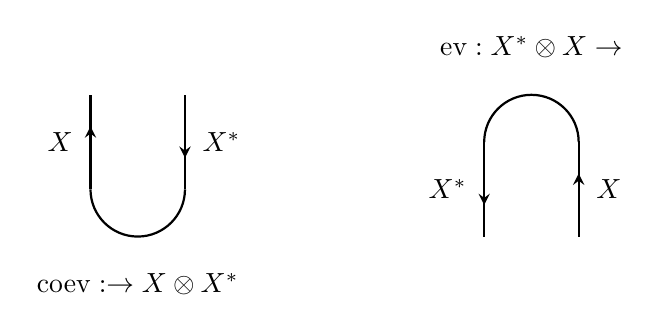
\begin{tikzpicture}[scale=1.0]
    % Cup (coevaluation): vacuum at bottom, pair created going up
    % U-shape opening downward, strands exit upward
    \begin{scope}[xshift=0cm]
        % The cup: arc at bottom connecting two upward strands
        \draw[thick] (-0.6,0.6) -- (-0.6,1.8);  % left strand going up
        \draw[thick] (0.6,0.6) -- (0.6,1.8);    % right strand going up
        \draw[thick] (-0.6,0.6) arc (180:360:0.6);  % U-shape at bottom
        % Arrows: left strand X (up), right strand X* (down orientation = up arrow reversed)
        \draw[thick,->,>=stealth] (-0.6,1.0) -- (-0.6,1.4);  % X: arrow up
        \draw[thick,->,>=stealth] (0.6,1.4) -- (0.6,1.0);    % X*: arrow down
        \node[left] at (-0.7,1.2) {$X$};
        \node[right] at (0.7,1.2) {$X^*$};
        \node at (0,-0.6) {$\mathrm{coev}: \one \to X \otimes X^*$};
    \end{scope}

    % Cap (evaluation): pair comes in from below, annihilates to vacuum at top
    % Inverted U-shape (cap) at top
    \begin{scope}[xshift=5cm]
        % Two strands coming from below, meeting in a cap at top
        \draw[thick] (-0.6,0) -- (-0.6,1.2);    % left strand
        \draw[thick] (0.6,0) -- (0.6,1.2);      % right strand
        \draw[thick] (-0.6,1.2) arc (180:0:0.6);  % cap at top
        % Arrows: left is X* (down arrow), right is X (up arrow)
        \draw[thick,->,>=stealth] (-0.6,0.8) -- (-0.6,0.4);  % X*: arrow down
        \draw[thick,->,>=stealth] (0.6,0.4) -- (0.6,0.8);    % X: arrow up
        \node[left] at (-0.7,0.6) {$X^*$};
        \node[right] at (0.7,0.6) {$X$};
        \node at (0,2.4) {$\mathrm{ev}: X^* \otimes X \to \one$};
    \end{scope}
\end{tikzpicture}
\caption{Coevaluation (cup) and evaluation (cap) morphisms.}
\label{fig:cups-caps}
\end{figure}

\begin{figure}[ht]
\centering
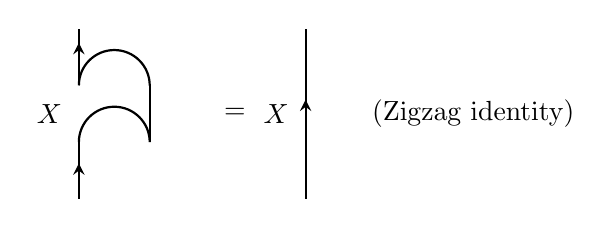
\begin{tikzpicture}[scale=0.9]
    % Zigzag: strand goes up, bends right (cup), goes down, bends left (cap), goes up
    % This is: id_X composed with (coev tensor id) composed with (id tensor ev)
    \begin{scope}[xshift=0cm]
        % Bottom segment going up
        \draw[thick] (0,0) -- (0,0.8);
        % Cup bending to the right
        \draw[thick] (0,0.8) arc (180:0:0.5);
        % Middle segment going down then up
        \draw[thick] (1,0.8) -- (1,1.6);
        % Cap bending back left
        \draw[thick] (1,1.6) arc (0:180:0.5);
        % Top segment going up
        \draw[thick] (0,1.6) -- (0,2.4);
        % Arrow on bottom segment
        \draw[thick,->,>=stealth] (0,0.2) -- (0,0.5);
        % Arrow on top segment
        \draw[thick,->,>=stealth] (0,1.9) -- (0,2.2);
        % Label
        \node[left] at (-0.1,1.2) {$X$};
    \end{scope}

    % Equals sign
    \node at (2.2,1.2) {$=$};

    % Straight line (identity)
    \begin{scope}[xshift=3.2cm]
        \draw[thick] (0,0) -- (0,2.4);
        \draw[thick,->,>=stealth] (0,1.0) -- (0,1.4);
        \node[left] at (-0.1,1.2) {$X$};
    \end{scope}

    % Label
    \node[right] at (4.0,1.2) {(Zigzag identity)};
\end{tikzpicture}
\caption{The zigzag identity: a bent string straightens to the identity.}
\label{fig:zigzag}
\end{figure}

\begin{definition}[Quantum dimension via loop]\label{def:quantum-dim-loop}
The quantum dimension $d_X$ of a simple object $X$ equals the value of a closed loop:
\begin{equation}
    d_X = \mathrm{ev}_X \circ \mathrm{coev}_X = \bigcirc_X
\end{equation}
Diagrammatically, closing a string labelled $X$ into a loop evaluates to the scalar $d_X \in k$.
\end{definition}

\begin{figure}[ht]
\centering
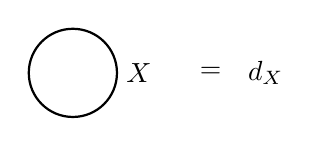
\begin{tikzpicture}[scale=0.7]
    % Loop
    \draw[thick] (0,0) circle (0.8);
    \node at (1.2,0) {$X$};

    % Equals
    \node at (2.5,0) {$=$};

    % Scalar
    \node at (3.5,0) {$d_X$};
\end{tikzpicture}
\caption{A closed loop evaluates to the quantum dimension.}
\label{fig:loop-qdim}
\end{figure}

\subsection{F-Moves and R-Moves Diagrammatically}\label{sec:F-R-moves}

\begin{definition}[F-move]\label{def:F-move}
The \emph{F-move} is the graphical representation of the associator. For simple objects $a, b, c, d$ with intermediate channels $e, f$:
\begin{equation}
    \fuselefttree{a}{b}{e}{c}{d} = \sum_f (F_{abc}^d)_e^f \; \fuserighttree{a}{b}{f}{c}{d}
\end{equation}
The F-symbol $(F_{abc}^d)_e^f$ (with multiplicity indices suppressed) gives the change-of-basis coefficient.
\end{definition}

\begin{definition}[R-move]\label{def:R-move}
For a braided category, the \emph{R-move} (braiding) exchanges two adjacent strands:
\begin{equation}
    \begin{tikzpicture}[baseline={(0,0.3)},scale=0.5]
        \begin{knot}[clip width=4]
            \strand[thick] (0,0) to[out=up,in=down] (1,1.5);
            \strand[thick] (1,0) to[out=up,in=down] (0,1.5);
        \end{knot}
        \node[below] at (0,0) {\small $a$};
        \node[below] at (1,0) {\small $b$};
    \end{tikzpicture}
    \;=\; R_{ab}^c \cdot
    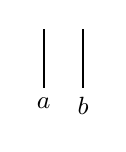
\begin{tikzpicture}[baseline={(0,0.3)},scale=0.5]
        \draw[thick] (0,0) -- (0,1.5);
        \draw[thick] (1,0) -- (1,1.5);
        \node[below] at (0,0) {\small $a$};
        \node[below] at (1,0) {\small $b$};
    \end{tikzpicture}
\end{equation}
where the crossing indicates which strand passes over (the R-symbol depends on total charge $c \in a \otimes b$).
\end{definition}

\begin{remark}[Pentagon and hexagon identities]
The F-symbols must satisfy the \emph{pentagon identity}: five ways to re-associate $(a \otimes b) \otimes c) \otimes d$ form a commuting pentagon. For braided categories, the \emph{hexagon identities} relate F-moves and R-moves, ensuring consistency of braiding with associativity.
\end{remark}

\subsection{Normalisation Choices}\label{sec:normalisation}

\begin{convention}[Normalisation]\label{conv:normalisation}
We adopt the following normalisation conventions throughout this paper:
\begin{enumerate}
    \item \textbf{Trivalent vertices:} Fusion vertices $v_{ab}^{c,\mu}: a \otimes b \to c$ (with multiplicity index $\mu$) are normalised so that
    \begin{equation}
        \sum_\mu (v_{ab}^{c,\mu})^\dagger v_{ab}^{c,\mu} = \mathrm{id}_{(a \otimes b) \to c}
    \end{equation}

    \item \textbf{Quantum dimensions:} $d_\one = 1$ (vacuum has unit dimension).

    \item \textbf{Closed loops:} A closed loop labelled $X_i$ evaluates to $d_i$:
    \begin{equation}
        \bigcirc_{X_i} = d_i
    \end{equation}

    \item \textbf{F-symbols:} For unitary fusion categories, F-symbols are unitary:
    \begin{equation}
        \sum_f (F_{abc}^d)_e^f \overline{(F_{abc}^d)_{e'}^f} = \delta_{e,e'}
    \end{equation}

    \item \textbf{R-symbols:} For unitary braided categories, R-symbols are unitary:
    \begin{equation}
        (R_{ab}^c)^\dagger R_{ab}^c = 1
    \end{equation}
\end{enumerate}
\end{convention}

\begin{remark}
These conventions are compatible with TensorCategories.jl defaults. Any discrepancies with specific literature sources will be documented case-by-case in the relevant sections.
\end{remark}

\subsection{Algebraic vs Diagrammatic Correspondence}\label{sec:alg-diag-correspondence}

\begin{claim}[Equivalence of calculi]\label{claim:calculus-equiv}
The diagrammatic calculus is equivalent to algebraic definitions:
\begin{center}
\begin{tabular}{ll}
\toprule
\textbf{Algebraic} & \textbf{Diagrammatic} \\
\midrule
Morphism $f: A \to B$ & Box with $A$ below, $B$ above \\
Composition $g \circ f$ & Vertical stacking \\
Tensor $f \otimes g$ & Horizontal juxtaposition \\
Associator $\alpha_{a,b,c}$ & F-move \\
Braiding $c_{a,b}$ & R-move (crossing) \\
Dual $X^*$ & Reversed strand direction \\
$\mathrm{coev}: \one \to X \otimes X^*$ & Cup (U-shape) \\
$\mathrm{ev}: X^* \otimes X \to \one$ & Cap (inverted U) \\
Trace $\mathrm{Tr}(f)$ & Close strand into loop \\
\bottomrule
\end{tabular}
\end{center}
\end{claim}

\begin{remark}
The diagrammatic calculus is more than mere notation: Mac Lane's coherence theorem ensures that any two ways of re-associating yield the same morphism when expressed via F-moves. This makes the graphical calculus a rigorous computational tool.
\end{remark}

\begin{citationblock}
Etingof--Gelaki--Nikshych--Ostrik, \emph{Tensor Categories}, AMS (2015), Ch.~2 and Ch.~4 \cite{EGNO2015} \unverified
\end{citationblock}
